\subsection{Le laboratoire et ses relations institutionnelles}
Le Laboratoire de l'Informatique du Parallélisme (abrégé \gls{lip}) est un laboratoire de recherche en informatique situé principalement sur le site Monod de l'École Normale Supérieure de Lyon.

\subsubsection{Présentation générale}
Créé dans les années 80, le Laboratoire de L'Informatique du Parallélisme devient \gls{ura} (URA) de l'\gls{ens} Lyon en 1989, puis \gls{umr} (UMR) en 1999 qui sera complété par l'Université Claude Bernard Lyon 1 en 2003. Le laboratoire est très tôt épaulé par l'Institut national de recherche en informatique et en automatique (\gls{inria}) qui est le principal acteur de la recherche en informatique et mathématique en France depuis 1967. Ainsi le laboratoire héberge plusieurs équipes-projets communes avec l'\gls{inria}. \cite{reportHCERES}\\

Le laboratoire compte 57 enseignant titulaires et chercheurs, entre 40 et 50 doctorants ainsi qu'une vingtaine de personnes sur des postes non permanents. L'équipe d'administration et l'équipe technique quant-à-elles sont épaulés par 12 ingénieurs.\\

Le \gls{lip} possède une bonne visibilité de ses équipes au niveau national et de plusieurs de ses membres au niveau international. Il occupe une place central dans le paysage de la recherche en informatique français pour quasiment l'ensemble de ses thématiques. La forte croissance du laboratoire lui a même obligé a s'étendre sur 2 autres sites : au sein de l’Institut Rhône-Alpin des Systèmes Complexes, et au sein de locaux appartenant à l’UCB à Gerland.

\subsubsection{Organisation générale}
Le laboratoire compose l'\gls{umr} 5668 avec l'ENS Lyon (EnsL), l'Université Claude Bernard Lyon 1, l'\gls{inria} et le CNRS. Il est dirigé par \textbf{M. Patrick Baillot} qui est secondé par \textbf{M. Frédéric Vivien}. Le responsable en charge de l'appel à projets, de la valorisation de recherche et des relations internationales est \textbf{M. Eddy Caron} et le responsable en charge des thèses, de l'enseignement et des postes non permanents est \textbf{M. Damien Stehlé}.

L'équipe administrative et l'équipe en charge des moyens informatique quant-à-elles sont composés de différentes personne issues des institutions qui constituent l'\gls{umr} 5668.\\

Le laboratoire héberge sept équipes de recherche dont cinq sont commune avec l'\gls{inria} : AriC, AVALON, CASH, DANTE, MC2, PLUME et ROMA chacune administrés par un chef d'équipe.

\begin{figure}[h]
	\center
	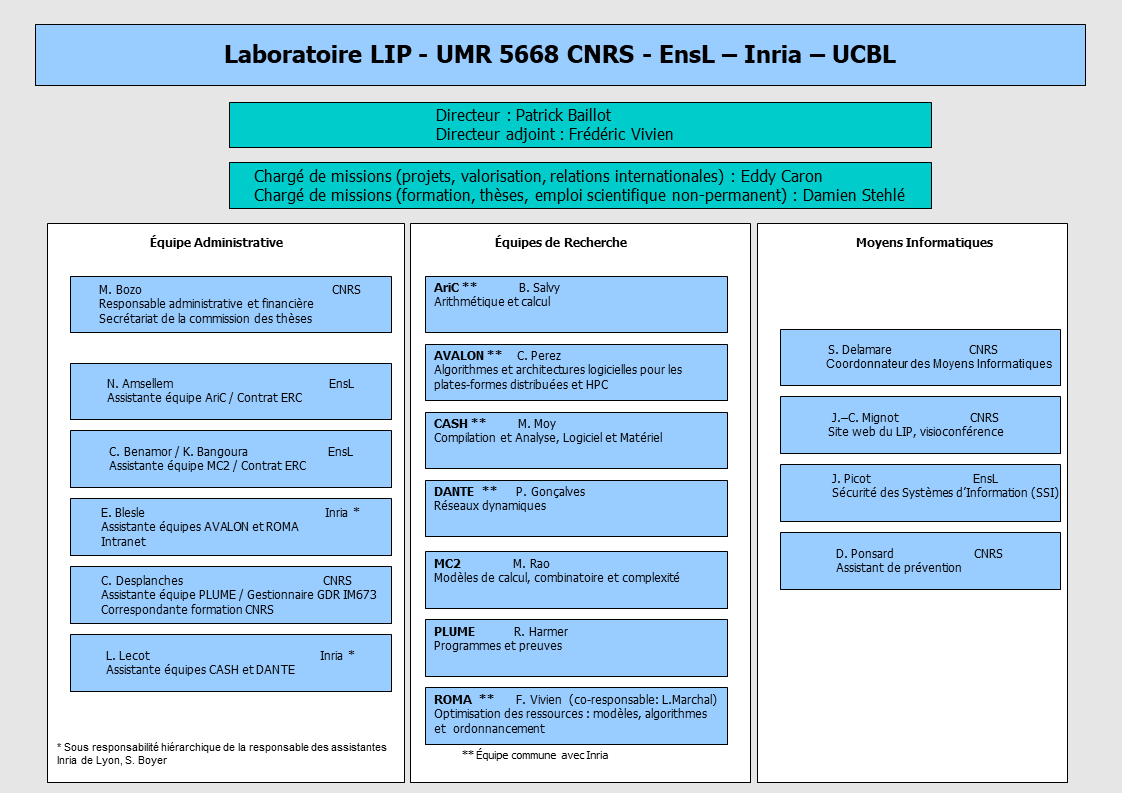
\includegraphics[scale=0.5]{partie1/images/organigramme.png}
	\caption{Organigramme du Laboratoire de l'Informatique du Parallélisme au 10 Avril 2018 \cite{organigramme}}
\end{figure}
\subsubsection{Des métiers variés}

\subsubsection{Le production du laboratoire}
